\documentclass[9pt]{beamer}
\usetheme[progressbar=head,numbering=fraction]{metropolis}
\usepackage[utf8]{inputenc}
\usepackage[T1]{fontenc}
\usepackage{lmodern}

\usepackage{empheq}
\makeatletter
\colorlet{shadecolour}{blue!30}
\newcommand\Ashaded[1]{\let\bgroup{\romannumeral-`}\@Ashaded#1&&\ENDDNE}
\def\@Ashaded#1&#2&#3\ENDDNE{%
\ifnum0=`{}\fi \setbox \z@
\hbox{$\displaystyle#1{}\m@th$\kern\fboxsep \kern\fboxrule }%
\edef\@tempa {\kern \wd\z@ &\kern -\the\wd\z@ \fboxsep
\the\fboxsep }\@tempa \colorbox{shadecolour}{$#1#2 $}%
}
\colorlet{bgcolour}{yellow!20}
\colorlet{rulecolour}{blue!30}
\newcommand\Acolorboxed[1]{\let\bgroup{\romannumeral-`}\@Acolorboxed#1&&\ENDDNE}
\def\@Acolorboxed#1&#2&#3\ENDDNE{%
  \ifnum0=`{}\fi \setbox \z@
    \hbox{$\displaystyle#1{}\m@th$\kern\fboxsep \kern\fboxrule }%
    \edef\@tempa {\kern \wd\z@ &\kern -\the\wd\z@ \fboxsep
        \the\fboxsep\fboxrule \the\fboxrule }\@tempa \fcolorbox{rulecolour}{bgcolour}{$ #1#2 $}%
}
\makeatother

\usepackage{amsfonts,amsmath}
\allowdisplaybreaks


%% X color
\definecolor{darkblueX}{RGB}{0,62,92}
\definecolor{lightblueX}{RGB}{0,104,128}
\definecolor{verylightblueX}{RGB}{212,232,239}
\definecolor{redX}{RGB}{169,32,33}




%% Font

\setbeamerfont{framesubtitle}{size=\tiny}
\setbeamerfont{alerted text}{shape=\bfseries}


\definecolor{lightr}{RGB}{204,0,0}
\newcommand{\eqsp}{\,}

%\usepackage[export]{adjustbox}

% Tighter itemize
\expandafter\def\expandafter\normalsize\expandafter{%
    \normalsize%
    \setlength\abovedisplayskip{1pt}%
    \setlength\belowdisplayskip{1pt}%
    \setlength\abovedisplayshortskip{1pt}%
    \setlength\belowdisplayshortskip{1pt}%
}

\expandafter\def\expandafter\small\expandafter{%
    \small%
    \setlength\abovedisplayskip{1pt}%
    \setlength\belowdisplayskip{1pt}%
    \setlength\abovedisplayshortskip{1pt}%
    \setlength\belowdisplayshortskip{1pt}%
}

%\usepackage{beamerX}
\newcommand{\alertmath}[1]{\textcolor{blue}{\boldsymbol{#1}}}
%\setboolean{displaylogo}{false}

\AtBeginSection[]
{
\begin{frame}
        \frametitle{Outline}
        \tableofcontents[currentsection]
   \end{frame}
}
\AtBeginSubsection[]
{
\begin{frame}
        \frametitle{Outline}
        \tableofcontents[currentsection,currentsubsection]
   \end{frame}
}

\setbeamertemplate{frametitle continuation}[from second][]

\usepackage{graphicx}%

\newcommand{\parinc}[2]{\parbox[c]{#1}{\includegraphics[width=#1]{#2}}}
\newcommand{\parinch}[3]{\parbox[c][#2]{#1}{\includegraphics[width=#1]{#3}}}
\newcommand{\parincb}[3]{\parbox[c]{#1}{\includegraphics[width=#1,height=#2]{#3}}}

\usepackage{color}
\newcommand{\red}[1]{\textcolor{red}{#1}}

\usepackage{tikz}


\usepackage{scalerel,stackengine}
\stackMath
\newcommand\reallywidehat[1]{%
\savestack{\tmpbox}{\stretchto{%
  \scaleto{%
    \scalerel*[\widthof{\ensuremath{#1}}]{\kern-.6pt\bigwedge\kern-.6pt}%
    {\rule[-\textheight/2]{1ex}{\textheight}}%WIDTH-LIMITED BIG WEDGE
  }{\textheight}% 
}{0.5ex}}%
\stackon[1pt]{#1}{\tmpbox}%
}

\newcommand{\grad}{\nabla}
\newcommand{\ind}[1]{\mathbf{1}_{#1}}

\DeclareMathOperator{\limSup}{limsup}%
\DeclareMathOperator{\limInf}{liminf}%
\DeclareMathOperator*{\argmax}{argmax}%
\DeclareMathOperator*{\argmin}{argmin}%
\DeclareMathOperator*{\supp}{Supp}%
\DeclareMathOperator{\pen}{pen}
\DeclareMathOperator{\dom}{dom}
\DeclareMathOperator{\price}{price}
\DeclareMathOperator{\sign}{sign}
\DeclareMathOperator{\KL}{KL}
\DeclareMathOperator{\Proj}{Proj}
\DeclareMathOperator{\Span}{span}


\DeclareMathOperator*{\tr}{tr}
\DeclareMathOperator*{\ra}{rank}
\DeclareMathOperator*{\conv}{conv}
\DeclareMathOperator{\ve}{vec}
\DeclareMathOperator{\diag}{diag}



\newcommand{\Espe}{\mathbb{E}}
\newcommand{\Vari}{\mathbb{V}}
\newcommand{\Cova}{\mathbb{C}\text{ov}}
\newcommand{\Prob}[2][]{\mathds{P}_{#1}\left\{#2\right\}}
\newcommand{\Esp}[2][]{\Espe_{#1}\left[#2\right]}
\newcommand{\Var}[2][]{\Vari_{#1}\left[#2\right]}
\newcommand{\Cov}[2][]{\Cova_{#1}\left[#2\right]}
\newcommand{\ud}{\textup{d}}
\newcommand{\charac}{\mathbf{1}}

\newcommand{\vecX}{\textbf{X}}
\newcommand{\vecx}{\textbf{x}}
\newcommand{\transp}[1]{{#1}^t}

\usepackage{pdfpages}
\usepackage{tikz}
\usepackage{dsfont}
\usepackage{ragged2e}
\usepackage{mathabx}
\usepackage[style=alphabetic, citestyle = authoryear, maxcitenames=2,backend=biber]{biblatex}
\addbibresource{../deeplearning_course.bib}
%Compile pdflatex, biber, pdflatex, pdflatex

\usepackage{graphicx}
\graphicspath{{}}
\usepackage{ragged2e}

\newcommand\citem[1]{{\scriptsize[\citetitle{#1}, \cite{#1}]}}
\DeclareMathOperator{\prox}{prox}
\newcommand{\eps}{\varepsilon}
\newcommand{\norm}[1]{\|#1\|}
\newcommand{\inr}[1]{\langle #1 \rangle}
\newcommand\redd[1]{\textcolor{red}{#1}}
\newcommand\blue[1]{\textcolor{blue}{#1}}
\newcommand\iid{\textit{i.i.d.}}
\newcommand\bW{\textbf{W}}
\newcommand\R{\mathds{R}}
\newcommand\bx{\mathbf{x}}
\renewcommand\pen{\textrm{pen}}
\newcommand{\E}{\mathds{E}}
\newcommand{\V}{\mathds{V}}
\newcommand{\cov}{\mathds{C}}
\renewcommand{\P}{\mathds{P}}

\usepackage{ifthen}
\newboolean{correction_bool}
\setboolean{correction_bool}{false}
\newcommand{\ifinclude}[1]{\ifthenelse{\boolean{correction_bool}}{#1}{}}


\title[Introduction to machine learning]{MSc Big Data for Business - {\em MAP 534} \\
Introduction to machine learning\\}

\author{}
\date{}

\begin{document}

\author[S. Le Corff]{\textcolor{violet}{Supervised classification (II)}\\ {\em {\small \textcolor{violet}{Logistic regression \& feed forward neural networks}}}}

\begin{frame}
\titlepage
\end{frame}

\section{Introduction}
\begin{frame}{Classification}

\textcolor{violet}{{\bf Setting}}

$\rightharpoondown$ Historical data  about \alert{individuals $i=1, \ldots, n$}.

$\rightharpoondown$ \textbf{Features} vector $X_i \in \R^d$ for each individual $i$.

$\rightharpoondown$ For each $i$, the individual \alert{belongs to a group} ($Y_i = 0$) or not ($Y_i = 1$).

$\rightharpoondown$ $Y_i \in \{ 0, 1 \}$ is  the \textbf{label} of $i$.


\vspace{.6cm}

\textcolor{violet}{{\bf Aim}}

$\rightharpoondown$ Given a new $X$ (with no corresponding label), \alert{predict a label in $\{ 0, 1 \}$}.

$\rightharpoondown$ Use data $\mathcal{D}_n = \{ (x_1, y_1), \ldots, (x_n, y_n) \}$ \alert{to construct a  \textbf{classifier}}.

\end{frame}

\begin{frame}
\frametitle{Best Solution}

\alert{The best solution} $f^*$ (which is independent of $\mathcal{D}_n$) is 

\begin{align*}
\Acolorboxed{f^* &= \arg\min_{f \in \mathcal{F}} R(f) = \arg\min_{f \in \mathcal{F}}
	\Esp{\mathds{1}_{Y\neq f(X)}} =  \arg\min_{f \in \mathcal{F}}
	\mathbb{P}(Y\neq f(X))\,.}
\end{align*}

\vspace{.3cm}

\textcolor{violet}{{\bf Bayes Predictor (explicit solution)}}

$\rightharpoondown$ \alert{Binary classification} with $0-1$ loss: 
			\begin{align*}
			f^*(\textbf{X}) = \begin{cases}
			+1 & \text{if  \, $\Prob{Y=1\middle|\textbf{X}} \geqslant \Prob{Y=0\middle| \textbf{X}}$}\\
			& \text{ $\Leftrightarrow \Prob{Y=1\middle|\textbf{X}} \geqslant 1/2$}\,,\\
			0  & \text{otherwise}\,.
			\end{cases}
			\end{align*}

\vspace{.3cm}

The explicit solution requires to \alert{know the conditional law of $Y$ given $X$}...

\end{frame}

\begin{frame}
  \frametitle{How to estimate the conditional law of $Y$?}


\textcolor{violet}{{\bf Fully parametric modeling.}}
    
     Estimate the law of $(\vecX,Y)$
      and use the \textbf{Bayes formula} to deduce an estimate of
      the conditional law of $Y$: \emph{LDA/QDA, Naive Bayes...}

\vspace{.3cm}

\textcolor{violet}{{\bf Parametric conditional modeling.}}
    
     Estimate the conditional law of
      $Y$ by a \textbf{parametric} law: \emph{linear regression, logistic regression, Feed Forward Neural Networks...}

\vspace{.3cm}

\textcolor{violet}{{\bf Nonparametric conditional modeling.}}
    
     Estimate the conditional  law of
      $Y$ by a \textbf{non parametric} estimate: \emph{kernel
        methods, nearest neighbors...}

 
\end{frame}


\begin{frame}\frametitle{Fully parametric modeling - Discriminant Analysis}


The \alert{conditional densities are modeled as multivariate normal}. For all class $k$, conditionnally on $\{Y=k\}$,
\begin{align*}
\vecX\sim \mathcal{N}(\mu_k, \Sigma_k)\,.
\end{align*}
\textcolor{lightr}{Discriminant functions}:
$$
g_k(\vecX) = \ln (\mathbb{P}\{\vecX|Y=k\}) + \ln(\Prob{Y=k})
\eqsp.
$$

In a two-classes problem, the optimal classifier is (\alert{see exercises}):

\begin{align*}
\Acolorboxed{&
f^*:x\mapsto \mathds{1}\{g_1(x)>g_{-1}(x)\}\eqsp.}
\end{align*}


\vspace{.2cm}


\textcolor{violet}{QDA (differents $\Sigma_k$ in each class)}  and \textcolor{violet}{LDA ($\Sigma_k=\Sigma$ for all $k$)} 

In the LDA case, the classification rule is of the form:
\begin{equation*}
f^*(x) = 1 \Leftrightarrow \langle w,x \rangle + b \geqslant 0\,,
\end{equation*}
where $w$ and $b$ depends on the model parameters.

 %$\rightharpoondown$ May lead to poor results is the \alert{model does not describe the data correctly}.


\end{frame}

%\begin{frame}{Coronary heart disease example}
%$\rightharpoondown$ \alert{Sample of males in a heart-disease high-risk region} (Western Cape, South Africa). 
%
%$\rightharpoondown$ \alert{Many covariates}.
%
%%\begin{verbatim}
%{\bf\textcolor{violet}{sbp}},	    	systolic blood pressure.
%
%{\bf\textcolor{violet}{tobacco}},		cumulative tobacco (kg).
%
%{\bf\textcolor{violet}{ldl}},		    low density lipoprotein, bad cholesterol. 
%
%{\bf\textcolor{violet}{famhist}},		family history of heart disease.
%
%{\bf\textcolor{violet}{typea}},		    type-A behavior.
%
%
%{\bf\textcolor{violet}{alcohol}},		current alcohol consumption.
%
%{\bf\textcolor{violet}{age}},		    age.
%
%{\bf\textcolor{violet}{chd}},		    response, coronary heart disease.
%%\end{verbatim}
%
%\end{frame}
%
%
%
%\begin{frame}{Coronary heart disease example}
%
%{\bf\textcolor{violet}{Analysis}} 
%
%Understand which factors are linked to the desease - \alert{prevention}.
%	
%$\rightharpoondown$ Importance of the effect.
%
%$\rightharpoondown$ Positive or negative effect.
%
%$\rightharpoondown$ Significativity.
%
%{\bf\textcolor{violet}{Prediction}} 
%
%Predict, for a new patient, the risk to declare the desease - \alert{monitoring}.
%
%$\rightharpoondown$ Quality of the prediction.
%
%$\rightharpoondown$ Parcimonious model.
%
%\end{frame}
%
%\begin{frame}{Scoring}
%
%{\bf\textcolor{violet}{Credit Default, Credit Score, Bank Risk, Market Risk Management}}
%
%$\rightharpoondown$ \alert{Data}: client profile, client credit history...
%
%$\rightharpoondown$ \alert{Input}: client profile.
%
%$\rightharpoondown$ \alert{Output}: credit risk.
%
%
%{\bf\textcolor{violet}{Analysis}}
%
%Understand which factors in this dataset are linked to the default - \alert{customer analysis}.
%
%$\rightharpoondown$  Importance of the effect.
%
%$\rightharpoondown$  Positive or negative effect.
%
%$\rightharpoondown$  Significativity.
%
%
%{\bf\textcolor{violet}{Prediction}}
%
%Predict, for a new client, the risk to default - \alert{decision aid}.
%
%$\rightharpoondown$  Quality of the prediction.
%
%$\rightharpoondown$ Parcimonious model.
%
%\end{frame}
%

\section{Logistic regression}

%\subsection{Model}

\begin{frame}{Semi-parametric modelling - logistic regression}


$\rightharpoondown$ The objective is to \alert{predict the  label $Y\in\{0,1\}$} based on $X\in\mathbb{R}^d$.

$\rightharpoondown$ Logistic regression \alert{models the distribution of $Y$ given $X$}.

\vspace{.3cm}

{\bf\textcolor{violet}{The model}} 
\begin{equation*}
\P(Y = 1| X) = \sigma(\langle w,X \rangle + b)\,,
\end{equation*}
where $w \in \R^d$ is a vector of model \textbf{weights} and $b \in \R$ is the \textbf{intercept}, and where $\sigma$ is the \textbf{sigmoid} function.

\vspace{.3cm}
 
\begin{tabular}{cc}
	\begin{minipage}{0.4\textwidth}
		\begin{equation*}
		\sigma: z \mapsto \frac{1}{1 + e^{-z}}\,.
		\end{equation*}%    
	\end{minipage}
	&
	\begin{minipage}{0.4\textwidth}
		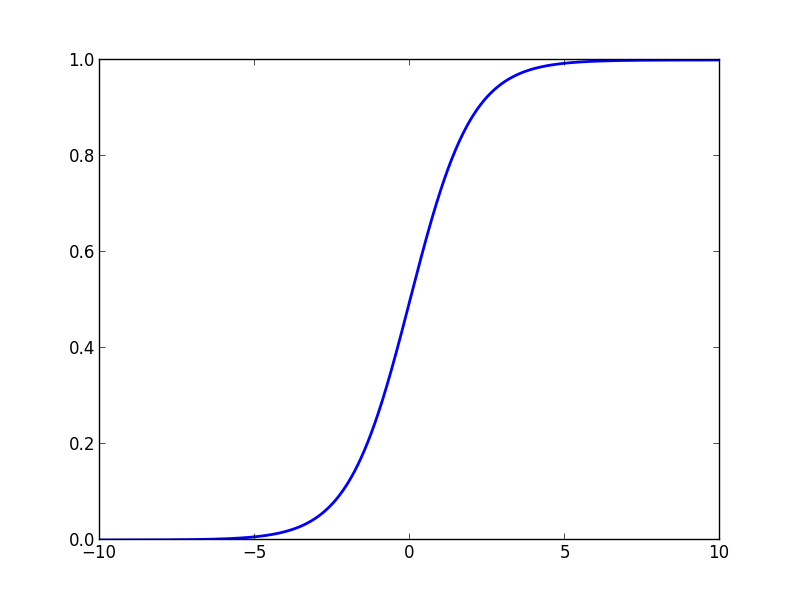
\includegraphics[width=4cm]{./sigmoid.png}  
	\end{minipage}    
\end{tabular}

$\rightharpoondown$ The sigmoid function is a \alert{model choice to map $\mathbb{R}$ into $(0,1)$}.

$\rightharpoondown$ Another widespread solution for $\sigma$ is $\sigma: z \mapsto  \P( Z \leqslant z)$ where $Z\sim \mathcal{N}(0,1)$, which leads to a \textbf{probit} regression model.

\end{frame}



\begin{frame}{Logistic regression}

{\bf\textcolor{violet}{Log-odd ratio}}

\begin{align*}
\Acolorboxed{&
\log \Big( \P(Y=1 | X)\Big) - \log \Big(\P(Y = 0| X) \Big) 
= \langle w,X \rangle  + b\,.}
\end{align*}

\vspace{.3cm}

{\bf\textcolor{violet}{Classification rule}}

 Note that 
\begin{equation*}
\P(Y = 1| X) \geq \P(Y = 0| X)
\end{equation*}
if and only if
\begin{equation*}
\langle w,x \rangle + b \geqslant 0\,.
\end{equation*}

$\rightharpoondown$ This is a \textbf{\alert{linear classification}} rule.

$\rightharpoondown$ This classifier requires to \alert{estimate $w$ and $b$}.

\end{frame}

\subsection{Inference}

\begin{frame}{Logistic regression}

$\rightharpoondown$   $\{(X_i,Y_i)\}_{1\leqslant i\leqslant n}$ are \alert{i.i.d. with the same distribution as $(X,Y)$}.

{\bf\textcolor{violet}{Likelihood}}

\begin{align*}
 \prod_{i=1}^n \P(Y_i | X_i) &= \prod_{i=1}^n \sigma(\langle w,X_i \rangle + b)^{Y_i} \big(1 - 
\sigma(\langle w,X_i \rangle + b) \big)^{1 - Y_i}\,, \\
& = \prod_{i=1}^n \sigma(\langle w,x_i \rangle + b)^{Y_i} 
\sigma(-\langle w,X_i \rangle - b)^{1 - Y_i}
\end{align*}
\smallskip

and the \alert{normalized negative loglikelihood} is 
\smallskip

\begin{equation*}
f(w,b) = \frac{1}{n}\sum_{i=1}^n \log (1 + \mathrm{e}^{-Y_i (\langle w,X_i \rangle + b)})= \frac{1}{n}\sum_{i=1}^n \ell(Y_i, \langle w,X_i \rangle + b)\,.
\end{equation*}
\end{frame}


\begin{frame}{Logistic regression}
		
Compute $\hat w_n$ and $\hat b_n$ as follows:

\begin{align*}
\Acolorboxed{&
(\hat w_n, \hat b_n) \in \argmin_{w \in \R^d, b \in \R}
\frac 1n \sum_{i=1}^n \log (1 + e^{-Y_i (\langle w,X_i \rangle + b)})\,.}
\end{align*}

\vspace{.3cm}

$\rightharpoondown$ It is an \textbf{average of losses}, one for each sample point.

$\rightharpoondown$ It is a \alert{convex and smooth problem}.


\medskip

Using the \textbf{\alert{logistic loss}} function
\smallskip 

\begin{equation*}
\ell: (y, y') \mapsto \log(1 + e^{-y y'}) 
\end{equation*}

yields

\begin{equation*}
(\hat w_n, \hat b_n) \in \argmin_{w \in \R^d, b \in \R}
\frac 1n \sum_{i=1}^n \ell(Y_i, \langle w,X_i \rangle + b)\,.
\end{equation*}
\end{frame}


\begin{frame}{Maximum likelihood estimate}
Assume for now that the intercept is 0. Then, the likelihood is,

$$
L_n(w)  =  \prod_{i=1}^n \left(\frac{e^{X_i^Tw}}{1+e^{X_i^T w}} \right)^{Y_i} \left(\frac{1}{1+e^{X_i^T w}} \right)^{1-Y_i} = \prod_{i=1}^n \left(\frac{e^{X_i^Tw Y_i}}{1+e^{X_i^T w}} \right)\,.
$$

And the \alert{negative $\log$-likelihood} is

\begin{align*}
\ell_n(w) = - \log(L_n(w)) =  \sum_{i=1}^n \left(-Y_i X_i^T w+ \log(1+ e^{X_i^Tw})\right)\,.
\end{align*}

{\bf\textcolor{violet}{Derivatives}}

%$$
%\nabla  \left(\log(L_n(\beta))\right)=   \left(\frac{\partial}{\partial \beta_0}(\beta),\cdots, \frac{\partial}{\partial \beta_d}(\beta)\right)\,. 
%$$

\begin{eqnarray*}
\frac{\partial \left(\log(L_n(w))\right)}{\partial w_j}&= &
\sum_{i=1}^n \left(Y_i X_{ij}
	- \frac{x_{ij} e^{X_i^T
	w}}{(1+ e^{X_i^T
	w})}   \right) \\
&=& \sum_{i=1}^n X_{ij} \left(Y_i - \sigma(\langle w,X_i \rangle)\right)\,.
\end{eqnarray*}

$\rightharpoondown$ \alert{No explicit solution} for the maximizer of the loglikelihood... Parameter estimate obtained using \alert{gradient based optimization} (see next lesson).

\end{frame}

\subsection{Intepretation}

\begin{frame}
The \alert{gradient of the negative loglikelihood} is, 

\begin{align*}
\Acolorboxed{&
\nabla \ell_n(w) = - \sum_{i=1}^n Y_i X_i + \sum_{i=1}^n \frac{\exp(\langle X_{i},w\rangle)}{1  + \exp(\langle X_{i},w\rangle)} X_i\,.}
\end{align*}

\vspace{.2cm}

On the other hand, for all $1\leqslant i \leqslant n$ and all $1 \leqslant j \leqslant d$,
\[
\partial_j \left( \frac{\exp(\langle X_{i},w\rangle)}{1  + \exp(\langle X_{i},w\rangle)} X_i \right) = \frac{\exp(\langle X_{i},w\rangle)}{(1  + \exp(\langle X_{i},w\rangle))^2} X_{ij}X_i\,,
\]
where $X_{ij}$ is the $j$th component of $X_i$. 

\vspace{.2cm}

Then, the \alert{Hessian matrix} is

\[
\big(H_n(w)\big)_{\ell j} = \sum_{i=1}^n \frac{\exp(\langle X_{i},w\rangle)}{(1  + \exp(\langle X_{i},w\rangle))^2} X_{ij}X_{i \ell}\,,
\]

that is,
\begin{align*}
\Acolorboxed{&
H_n(w) = \sum_{i=1}^n \frac{\exp(\langle X_{i},w\rangle)}{(1  + \exp(\langle X_{i},w\rangle))^2} X_{i} X^T_{i}\,.}
\end{align*}

\vspace{.3cm}

{\bf \textcolor{violet}{$H_n(\beta)$ is a semi positive definite matrix, which implies that $\ell_n(\beta)$ is convex}}.

\end{frame}

\begin{frame}{Asymptotic properties}


{\bf\textcolor{violet}{Assumptions}}

$\rightharpoondown$ \alert{$\widehat w_n\to w^*$ almost surely}. 

$\rightharpoondown$ There exists a continuous and nonsingular function $H$ such that \alert{$n^{-1}H_{n}(w)$ converges to $H(w)$}, uniformly in a ball around $w^*$.

\vspace{.5cm}

For all $t\in\R^d$, using a Taylor expansion,
\[
\mathbb{E} \left[ \exp\left( - \frac{1}{\sqrt{n}} \langle t, \nabla \ell_n(w^{\star}) \rangle \right) \right] \to_{n\to \infty}  \exp\Bigg( \frac{1}{2} t^T H(w^{\star}) t \Bigg)\,.
\]

Therefore, 
\begin{align*}
\Acolorboxed{& -\nabla \ell_n(w^{\star}) / \sqrt{n} \Rightarrow \mathcal{N}(0, H(w^{\star}))\,.}
\end{align*}

\vspace{.5cm}

On the other hand, by \alert{Slutsky lemma}, 

\begin{align*}
\Acolorboxed{&
\sqrt{n} (\widehat{w}_n - w^{\star}) \Rightarrow \mathcal{N}(0,  H(w^{\star})^{-1})\,.}
\end{align*}

\end{frame}

\begin{frame}{Confidence interval}

$\rightharpoondown$ $\sqrt{n} ( \widehat{w}_j - w^{\star}_j) $ \alert{converges in distribution to a centered Gaussian random variable with variance $(H(w^{\star})^{-1})_{jj}$}.

\vspace{.3cm}

Almost surely,
\begin{align*}
\widehat{\sigma}_{n,j}^2 = (n H_n(\widehat{w}_n)^{-1})_{jj} \to_{n\to \infty} (H(w^{\star})^{-1})_{jj}\,.
\end{align*}

Then, 

\begin{align*}
\Acolorboxed{&
\sqrt{\frac{n}{\widehat{\sigma}_{n,j}^2}} (\widehat{w}_{n,j} - \beta^{\star}_j ) \to_{n\to \infty} \mathcal{N}(0,1)\,.}
\end{align*}

\vspace{.2cm}

An \alert{asymptotic confidence interval $\mathcal{I}_{n,\alpha}$ of level $1-\alpha$} is then 



\begin{align*}
\Acolorboxed{&
\mathcal{I}_{n,\alpha} = \left[ \widehat{w}_{n,j} - z_{1-\alpha/2} \sqrt{\frac{\widehat{\sigma}^2_{n,j}}{n}}\,,\; \widehat{\beta}_{n,j} + z_{1-\alpha/2} \sqrt{\frac{\widehat{\sigma}^2_{n,j}}{n}}  \right]\,,}
\end{align*}

\vspace{.2cm}
where $z_{1- \alpha/2}$ is the quantile of order $1- \alpha/2$ of $\mathcal{N}(0, 1)$.
\end{frame}

%\begin{frame}{Test}
%
%\end{frame}
%
%\subsection{prediction}
%
%\begin{frame}{Test}
%
%\end{frame}


\section{Feed Forward Neural Networks}

\subsection{Model}

\begin{frame}{Softmax function}
$\rightharpoondown$ The objective is to \alert{predict the  label $Y\in\{1, \ldots, M\}$} based on $X\in\mathbb{R}^d$.

$\rightharpoondown$ Softmax regression \alert{models the distribution of $Y$ given $X$}.

\vspace{.3cm}

{\bf\textcolor{violet}{The model}} 

For all $1\leqslant m\leqslant M$,
\begin{align*}
z_m &= \langle w_m,X \rangle + b_m\,,\\
\P(Y = m| X) &= \mathrm{softmax}(z)_m\,,
\end{align*}

where $z\in\R^M$, $w_m \in \R^d$ is a vector of model \textbf{weights} and $b_m \in \R$ is an \textbf{intercept}, and where $\mathrm{softmax}$ is the \textbf{softmax} function: for all $1\leqslant m\leqslant M$,

$$
\mathrm{softmax}(z)_m = \frac{\mathrm{exp}(z_m)}{\sum_{j=1}^{M}\mathrm{exp}(z_j)}\,.
$$

\end{frame}

\begin{frame}{A neuron}

\begin{center}
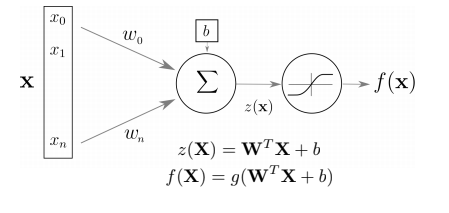
\includegraphics[width = 0.75\textwidth]{neuron.png}
\end{center}

$\rightharpoondown$ $X$ \alert{input in $\R^d$}.

$\rightharpoondown$ $z(X)$ \alert{pre-activation in $\R^M$}, with \alert{weight $W\in\R^{dxM}$} and \alert{bias $b\in\R^M$}.

$\rightharpoondown$ $g$ \alert{softmax function}.

\vspace{.3cm}

{\bf\textcolor{violet}{On neuron is a multi-class extension of the logistic regression model}}. 

\end{frame}

\begin{frame}{Layer of neurons and hidden states}

\begin{center}
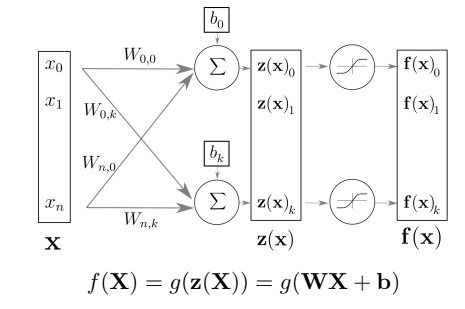
\includegraphics[width = 0.75\textwidth]{neuronlayer.png}
\end{center}

$\rightharpoondown$ $X$ \alert{input in $\R^d$}.

$\rightharpoondown$ $z(X)$ \alert{pre-activation in $\R^k$}, with \alert{weight $W\in\R^{dxk}$} and \alert{bias $b\in\R^k$}.

$\rightharpoondown$ $g$ \alert{any activation function} (nonlinear \& nondecreasing function).

$\rightharpoondown$ $f(X)$ \alert{hidden state} in $\R^k$ which may be used as input of a new neuron...


\end{frame}

\begin{frame}{Feed Forward Network}

\begin{center}
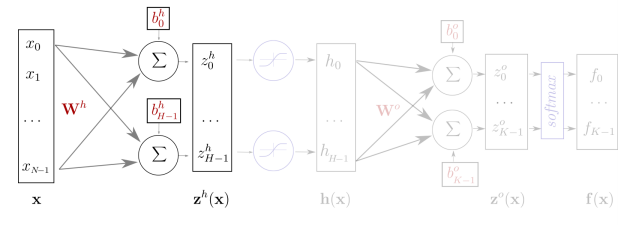
\includegraphics[width = 0.9\textwidth]{ffnn1.png}
\end{center}

$\rightharpoondown$ $X$ \alert{input in $\R^d$}.

$\rightharpoondown$ $z^h(X)$ \alert{pre-activation in $\R^H$}, with \alert{weight $W^h\in\R^{dxH}$} and \alert{bias $b^h\in\R^H$}.


\end{frame}

\begin{frame}{Feed Forward Network}

\begin{center}
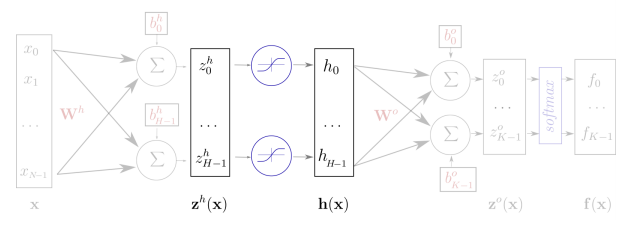
\includegraphics[width = 0.75\textwidth]{ffnn2.png}
\end{center}

$\rightharpoondown$ $X$ \alert{input in $\R^d$}.

$\rightharpoondown$ $z^h(X)$ \alert{pre-activation in $\R^H$}, with \alert{weight $W^h\in\R^{dxH}$} and \alert{bias $b^h\in\R^H$}.

$\rightharpoondown$ $g$ \alert{any activation function} to produce $h\in\R^H$.
\end{frame}

\begin{frame}{Feed Forward Network}

\begin{center}
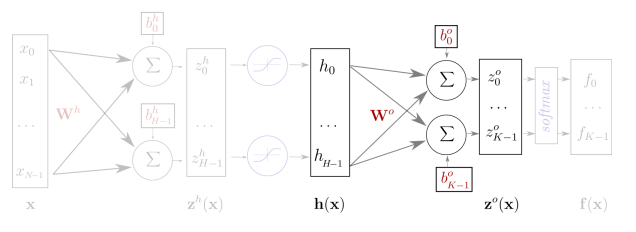
\includegraphics[width = 0.75\textwidth]{ffnn3.png}
\end{center}

$\rightharpoondown$ $X$ \alert{input in $\R^d$}.

$\rightharpoondown$ $z^h(X)$ \alert{pre-activation in $\R^H$}, with \alert{weight $W^h\in\R^{dxH}$} and \alert{bias $b^h\in\R^H$}.

$\rightharpoondown$ $g$ \alert{any activation function} to produce $h\in\R^H$.

$\rightharpoondown$ $z^o(X)$ \alert{pre-activation in $\R^M$}, with \alert{weight $W^o\in\R^{HxM}$} and \alert{bias $b^o\in\R^M$}.

\end{frame}

\begin{frame}{Feed Forward Network}

\begin{center}
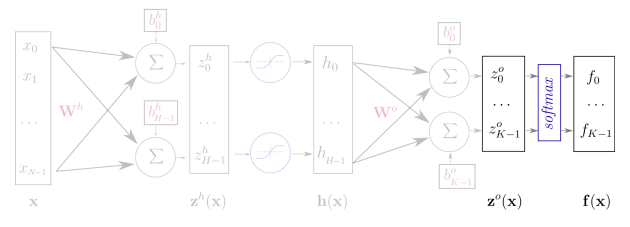
\includegraphics[width = 0.75\textwidth]{ffnn4.png}
\end{center}

$\rightharpoondown$ $X$ \alert{input in $\R^d$}.

$\rightharpoondown$ $z^h(X)$ \alert{pre-activation in $\R^H$}, with \alert{weight $W^h\in\R^{dxH}$} and \alert{bias $b^h\in\R^H$}.

$\rightharpoondown$ $g$ \alert{any activation function} to produce $h\in\R^H$.

$\rightharpoondown$ $z^o(X)$ \alert{pre-activation in $\R^M$}, with \alert{weight $W^o\in\R^{HxM}$} and \alert{bias $b^o\in\R^M$}.

$\rightharpoondown$  Apply the \alert{softmax function to produce the output}, i.e. $\mathbb{P}(Y=m|X)$ for $1\leqslant m \leqslant M$.
\end{frame}

\begin{frame}{Activation functions}

\begin{center}
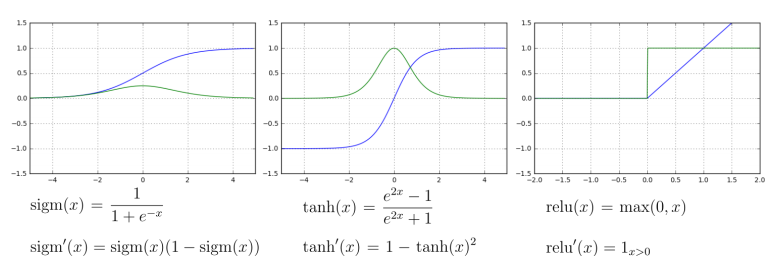
\includegraphics[width = 0.9\textwidth]{activations.png}
\end{center}

$\rightharpoondown$ As there is no modelling assumptions anymore, \alert{virtually any activation function} may be used. 

$\rightharpoondown$ The rectified linear unit (RELU) activation function $\sigma(x) = \mathrm{max}(0,x)$ and its extensions are the default recommendation in modern implementations  (Jarrettet al., 2009; Nair and Hinton, 2010; Glorot et al., 2011a), (Maas et al.,2013),  (He et al., 2015). One of the major motivations arise from the \alert{gradient based parameter optimization which is numerically more stable with this choice}. 

\end{frame}

\subsection{Implementation}

\begin{frame}{MNIST}

$\rightharpoondown$ This dataset contains images representing handwritten digits. Each image is made of \alert{$28$ x $28$ pixels}, and each pixel is represented by an integer (gray level). These arrays can be flattened into vectors in $\R^{784}$. 

$\rightharpoondown$ The \alert{labels in $\{0,\ldots,9\}$ are represented using one-hot-encoding} and grayscale of each pixel in $\{0,\ldots, 255\}$ are normalized to be in $(0,1)$.

\begin{figure}
\begin{center}
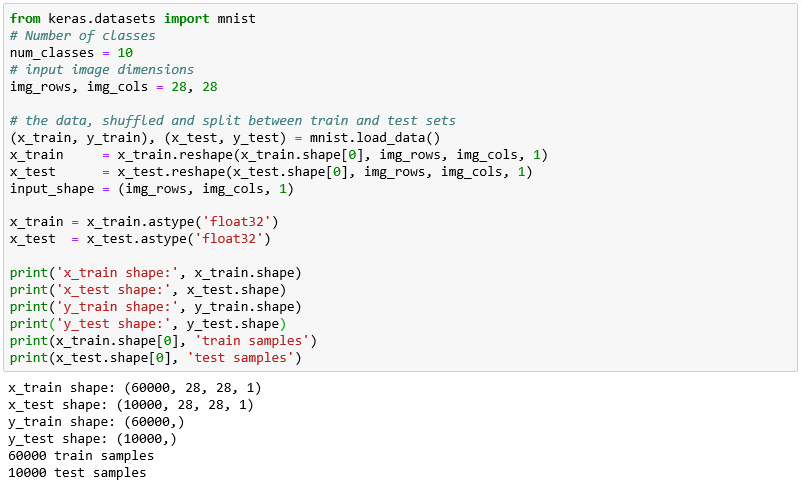
\includegraphics[width = .85\linewidth]{./MNIST_data1.png}
\end{center}
\end{figure}
\end{frame}

\begin{frame}{MNIST}

$\rightharpoondown$ This dataset contains images representing handwritten digits. Each image is made of \alert{$28$ x $28$ pixels}, and each pixel is represented by an integer (gray level). These arrays can be flattened into vectors in $\R^{784}$. 

$\rightharpoondown$ The \alert{labels in $\{0,\ldots,9\}$ are represented using one-hot-encoding} and grayscale of each pixel in $\{0,\ldots, 255\}$ are normalized to be in $(0,1)$.

\begin{figure}
\begin{center}
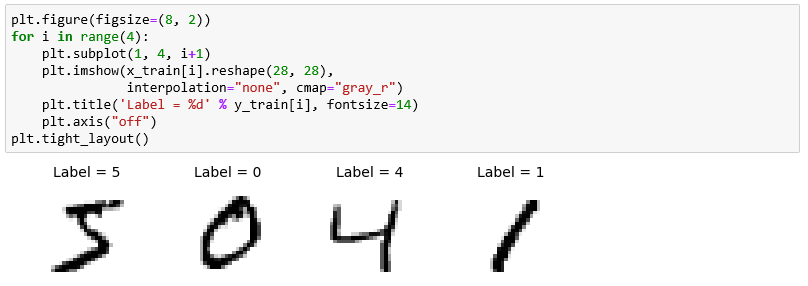
\includegraphics[width = .9\linewidth]{./MNIST_data2.png}
\end{center}
\end{figure}
\end{frame}

\begin{frame}{The model with Keras}
\begin{figure}
\begin{center}
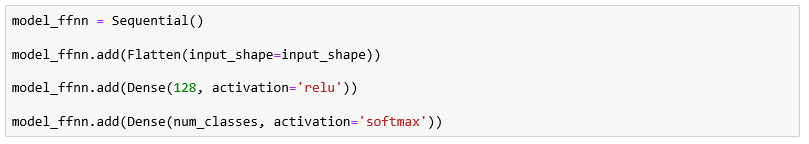
\includegraphics[width = .9\linewidth]{./MNIST_ffnn1.png}
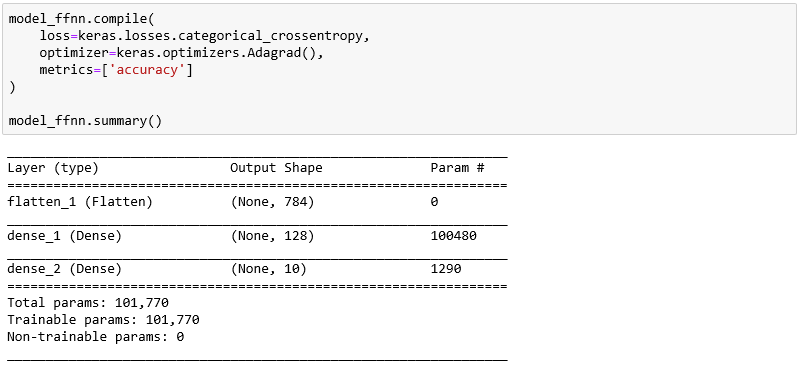
\includegraphics[width = .9\linewidth]{./MNIST_ffnn2.png}
\end{center}
\caption{Feed Forward Neural network. $h_1$ is obtained with the \alert{RELU activation function and is in $\R^{128}$}. The last layer is $h_2\in\R^{10}$ and is \alert{obtained with the softmax activation function} so that each component $m$ models $\mathbb{P}(Y=m|X)$. This neural network with one hidden layer relies on 101.770 parameters.}
\end{figure}
\end{frame}

\begin{frame}{Inference}
$\rightharpoondown$ This models relies on more than \alert{100.000 unknown parameters} which should be estimated. 

\vspace{.2cm}

$\rightharpoondown$ As for the logistic regression and the discriminant analysis, a common choice is to \alert{minimize the negative loglikelihood of the data}:
$$
\theta \mapsto -\frac{1}{n} \sum_{i=1}^n\sum_{k=1}^{10} \mathds{1}_{Y_i=k}\log \mathbb{P}_{\theta}(Y_i = k | X_i)\,.
$$

\vspace{.2cm}

$\rightharpoondown$ The negative loglikelihood is computed using $n = 60.000$ training samples and \alert{minimized using gradient descent algorithms} - \textcolor{violet}{see next lesson}. 

\vspace{.2cm}

$\rightharpoondown$ Then, the performance of the model is assessed using $10.000$ new (test) samples: the \alert{accuracy is the frequency of labels which are well predicted by the model with the estimated parameters}.


\end{frame}

\begin{frame}
\begin{figure}
\begin{center}
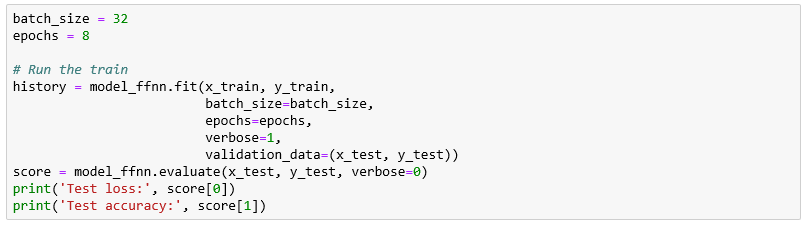
\includegraphics[width = .85\linewidth]{./MNIST_ffnn3.png}
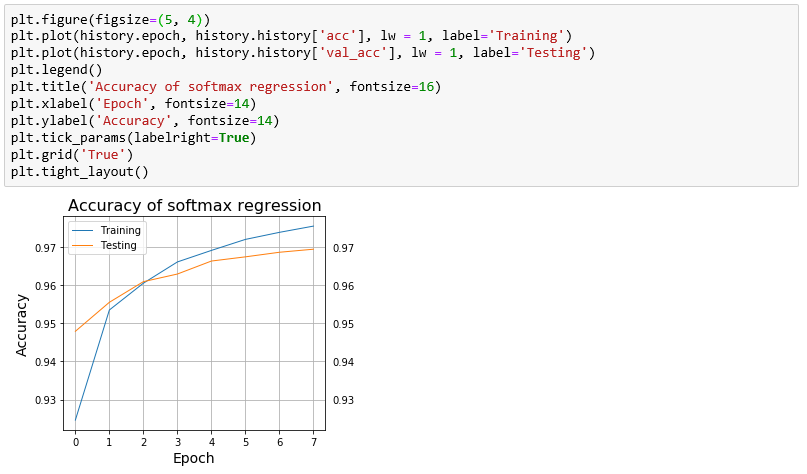
\includegraphics[width = .85\linewidth]{./MNIST_ffnn4.png}
\end{center}
\caption{Minimization of the negative liglikelihood using a gradient descent algorithm (here AdaGrad). The gradient is computed using batches of $32$ observations and the whole data set is used $8$ times.}
\end{figure}
\end{frame}


\end{document}


